\section{Experimental Setup}
\label{sec:exp_setup}

In this section, we elaborate on the experimental setup of our case studies. Our investigation spans two representative and distinct settings:
1) online reinforcement learning with 3D maze environments of DMLab~\citep{beattie2016deepmind}, and 2) imitation learning from mixed-quality human demonstrations of RoboMimic~\citep{mandlekar2021matters}. For each of them, we discuss task selection, baselines, and training and evaluation protocols.
Teasers of these tasks are shown in Figure~\ref{fig:tasks}.

\subsection{Task Settings and Environments}


\textbf{DeepMind Lab}~\citep{beattie2016deepmind} is a 3D learning environment with diverse tasks.
Agents spawn in visually complex worlds, receive ego-centric (thus partially observable) RGB pixel inputs, and execute joystick actions. We consider three levels from this benchmark: Goal Maze, Watermaze~\citep{watermaze}, and Sky Maze with Irreversible Path. They challenge agents to explore, memorize, and plan over a long horizon. Their goals are similar --- to navigate in complicated mazes and find a randomly spawned goal, upon which sparse rewards will be released.
Episodes start with randomly spawned agents and goals and terminate once goals are reached or elapsed steps have exceeded pre-defined horizons.

\textbf{RoboMimic}~\citep{mandlekar2021matters} is a framework designed for studying robot manipulation and learning from demonstrations. Agents control robot arms with fixed bases, receive proprioceptive measurements and image observations from mounted cameras, and operate with continuous control.
We evaluate two simulated tasks: ``Lift'' and ``Can''. In the ``Lift'' task, robots are tasked with picking up a small cube. In the ``Can'' task, robots are required to pick up a soda can from a large bin and place it into a smaller target bin.
Episodes start with randomly initialized object configuration and terminate upon successfully completing the task or exceeding pre-defined horizons.






\begin{table}[t!]
\caption{\textbf{Generalization gaps between training and testing for DMLab levels.} Note that agents resulting from task-difficulty-based curricula are not trained on test configurations. Therefore, their performance should be considered as \emph{zero-shot}.}
\label{table:dmlab_exp_setting}
\vspace{0.1in}
\centering
\resizebox{1\textwidth}{!}{
\begin{tabular}{@{}c|c|c|ccccc@{}}
\toprule
\multirow{2}{*}{\textbf{\begin{tabular}[c]{@{}c@{}}Level\\ Name\end{tabular}}} & \multirow{2}{*}{\textbf{\begin{tabular}[c]{@{}c@{}}Difficulty\\ Parameter\end{tabular}}} & \multirow{2}{*}{\textbf{\begin{tabular}[c]{@{}c@{}}Test\\ Difficulty\end{tabular}}} & \multicolumn{5}{c}{\textbf{Training Difficulty}}                                                                                                                                                                                                                                                                               \\ \cmidrule(l){4-8} 
                                                                               &                                                                                          &                                                                                     & \begin{tabular}[c]{@{}c@{}}Ours\\ (Learning Progress)\end{tabular} & \begin{tabular}[c]{@{}c@{}}Ours\\ (Task Difficulty)\end{tabular} & \begin{tabular}[c]{@{}c@{}}BC\\ w/ Expert Data\end{tabular} & \begin{tabular}[c]{@{}c@{}}RL\\ (Oracle)\end{tabular} & \begin{tabular}[c]{@{}c@{}}Curriculum RL\\ (Oracle)\end{tabular} \\ \midrule
Goal Maze                                                                      & Room Numbers                                                                             & 20                                                                                  & 20                                                                 & 5→10→15                                                          & 20                                                          & 20                                                    & 5→10→15→20                                                       \\
Watermaze                                                                      & Spawn Radius                                                                             & 580                                                                                 & 580                                                                & 150→300→450                                                      & 580                                                         & 580                                                   & 150→300→450→580                                                  \\
Irreversible Path                                                              & Built-In Difficulty                                                                      & .9                                                                                  & .9                                                                 & .1→.3→.5→.7                                                      & .9                                                          & .9                                                    & .1→.3→.5→.7→.9                                                   \\ \bottomrule
\end{tabular}

}
\end{table}


\subsection{Baselines}
The primary goal of these case studies is to assess the effectiveness of our proposed cross-episodic curriculum in increasing the sample efficiency and boosting the generalization capability of Transformer agents. Therefore, in online RL settings, we compare against source RL agents which generate training data for our method and refer to them as \textit{oracles}. These include a) PPO agents directly trained on test task distributions, denoted as ``\textbf{RL (Oracle)}'' hereafter, and b) curriculum PPO agents that are gradually adapted from easier tasks to the test difficulty, which is referred to as ``\textbf{Curriculum RL (Oracle)}''.
Furthermore, we compare against one concurrent and competitive method Agentic Transformer~\citep{liu2023emergent}, denoted as ``\textbf{AT}''. It is closely related to our method, training Transformers on sequences of trajectory ascending sorted according to their rewards.
We also compare against popular offline RL method Decision Transformer~\citep{chen2021decisiontransformer}, denoted as ``\textbf{DT}''.
Additionally, we include another behavior cloning agent that has the same model architecture as ours but is trained on optimal data without cross-episodic attention. 
This baseline is denoted as ``\textbf{BC w/ Expert Data}''.
For the case study on IL from mixed-quality demonstrations, we adopt the most competing approach, \textbf{BC-RNN}, from \citet{mandlekar2021matters} as the main baseline. We also include comparisons against other offline RL methods~\citep{levine2020offline} such as Batch-Constrained Q-learning~(\textbf{BCQ})~\citep{fujimoto2018offpolicy} and Conservative Q-Learning~(\textbf{CQL})~\citep{kumar2020conservative}.


\subsection{Training and Evaluation}
We follow the best practice to train Transformer agents, including adopting AdamW optimizer~\citep{loshchilov2019decoupled}, learning rate warm-up and cosine annealing~\citep{loshchilov17cosinelr}, etc.
Training is performed on NVIDIA V100 GPUs. 
During evaluation, for agents resulting from our method, each run involves several test rollouts to fill the context. We keep hidden states of Transformer-XL~\citep{dai2019transformerxl} propagating across episodes.
We run other baselines and oracles for 100 episodes to estimate their performances.
For our methods on RL settings, we compute the maximum success rate averaged across a sliding window over all test episodes to account for in-context improvement.
The size of the sliding window equals one-quarter of the total test episodes.
These values are averaged over 20 runs to constitute the final reporting metric.
For our methods on the IL setting, since all training data are successful trajectories, we follow \citet{mandlekar2021matters} to report the maximum success rate achieved over the course of training, directly averaged over test episodes.

\section{Experiments}
\label{sec:experiments}
\begin{figure}[!t]
\vspace{-0.1in}
    \centering
    \makebox[\textwidth][c]{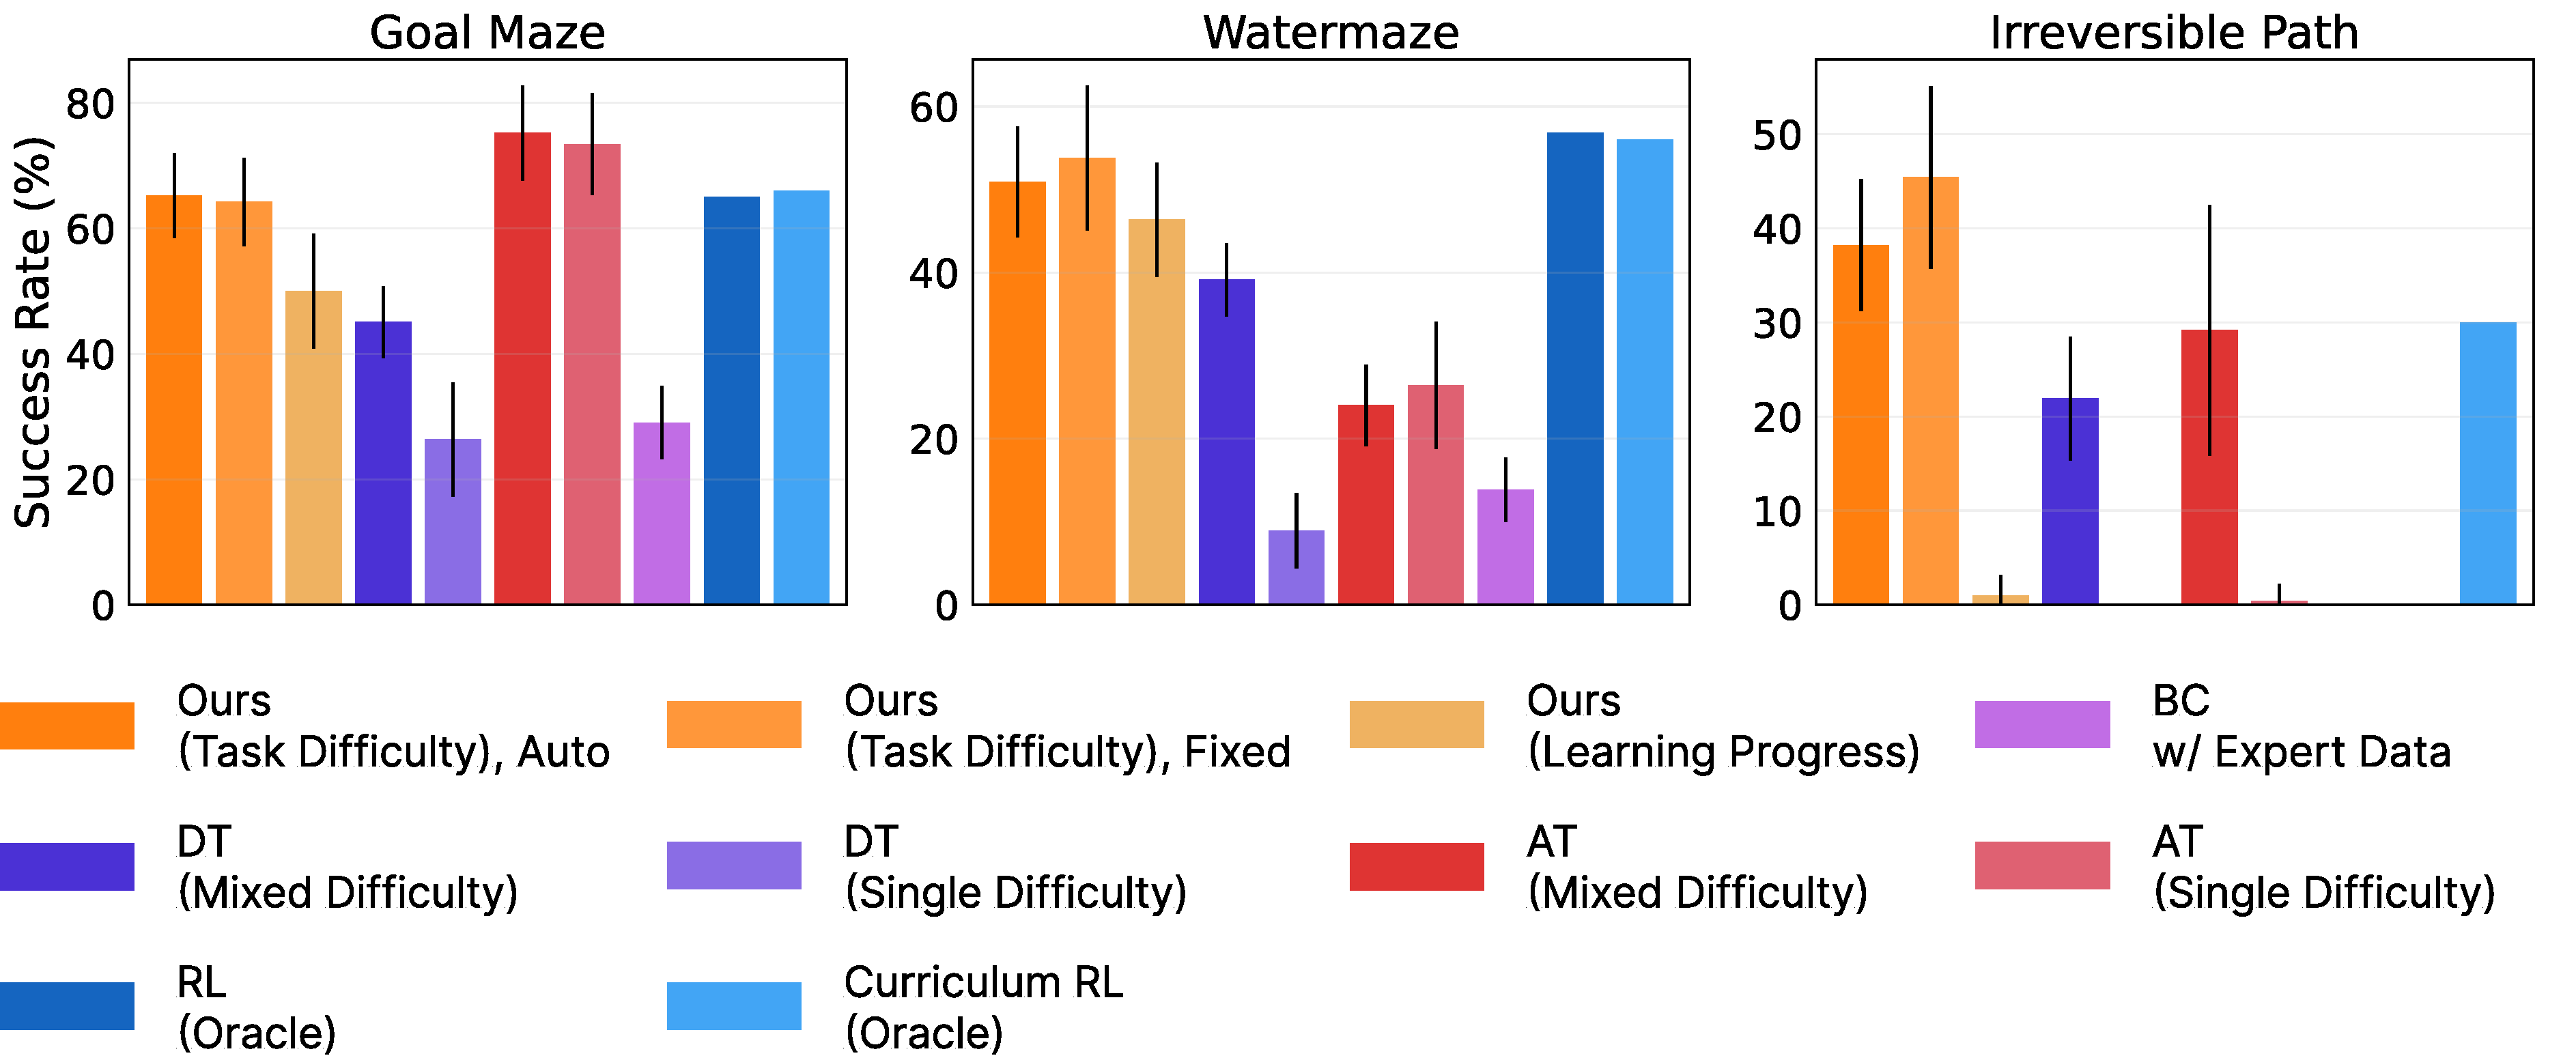
\includegraphics[width=1\textwidth]{fig/dmlab_main-fig.pdf}}
    \caption{\textbf{Evaluation results on DMLab.} Our \cec agents perform comparable to RL oracles and on average outperform other baseline methods. On the hardest task Irreversible Path where the RL oracle and BC baseline completely fail, our agents outperform the curriculum RL oracle by $50\%$ even in a \textit{zero-shot} manner. For our methods, DT, AT, and the BC w/ expert data baselines, we conduct 20 independent evaluation runs, each consisting of 100 episodes for Goal Maze and Watermaze and 50 episodes for Irreversible Path due to longer episode length. We test RL oracles for 100 episodes. The error bars represent the standard deviations over 20 runs.}
    \label{fig:dmlab_core}
    \vspace{-1em}
\end{figure}


We aim to answer the following four research questions through comprehensive experiments.

\begin{enumerate}
    \item{To what extent can our cross-episodic curriculum increase the sample efficiency of Transformer agents and boost their generalization capability?}

    \item{Is CEC consistently effective and generally applicable across distinct learning settings?}

    \item{What are the major components that contribute to the effectiveness of our method?}

\end{enumerate}


\vspace{-0.5em}

\subsection{Main Evaluations}
We answer the first two questions above by comparing learned agents from our method against 1) Reinforcement Learning (RL) oracles in online RL settings and 2) well-established baselines on learning from mixed-quality demonstrations in the Imitation Learning (IL) setting.

We first examine agents learned from learning-progress-based and task-difficulty-based curricula in challenging 3D maze environments.
The first type of agent is denoted as ``\textbf{Ours (Learning Progress)}''.
For the second type, to ensure that the evaluation also contains a series of tasks with increasing difficulty, we adopt two mechanisms that control the task sequencing~\citep{Narvekar2017AutonomousTS}: 1) fixed sequencing where agents try each level of difficulty for a fixed amount of times regardless of their performance and 2) dynamic sequencing where agents are automatically promoted to the next difficulty level if they consecutively succeed in the previous level for three times.
We denote these two variants as ``\textbf{Ours (Task Difficulty), Fixed}'' and ``\textbf{Ours (Task Difficulty), Auto}'', respectively.
Note that because the task-difficulty-based curriculum does not contain any training data on test configurations, these two settings are zero-shot evaluated on test task distributions. We summarize these differences in Table~\ref{table:dmlab_exp_setting}. 
We denote AT and DT trained on data consisting of a mixture of task difficulties as ``\textbf{AT (Mixed Difficulty)}'' and ``\textbf{DT (Mixed Difficulty)}''.
Note that these data are the same used to train ``Ours (Task Difficulty)''.
Similarly, we denote AT and DT directly trained on test difficulty as ``AT (Single Difficulty)'' and ``DT (Single Difficulty)''.
These data are the same used to train ``Ours (Learning Progress)''.
\begin{figure}[!t]
    \centering
    \makebox[\textwidth][c]{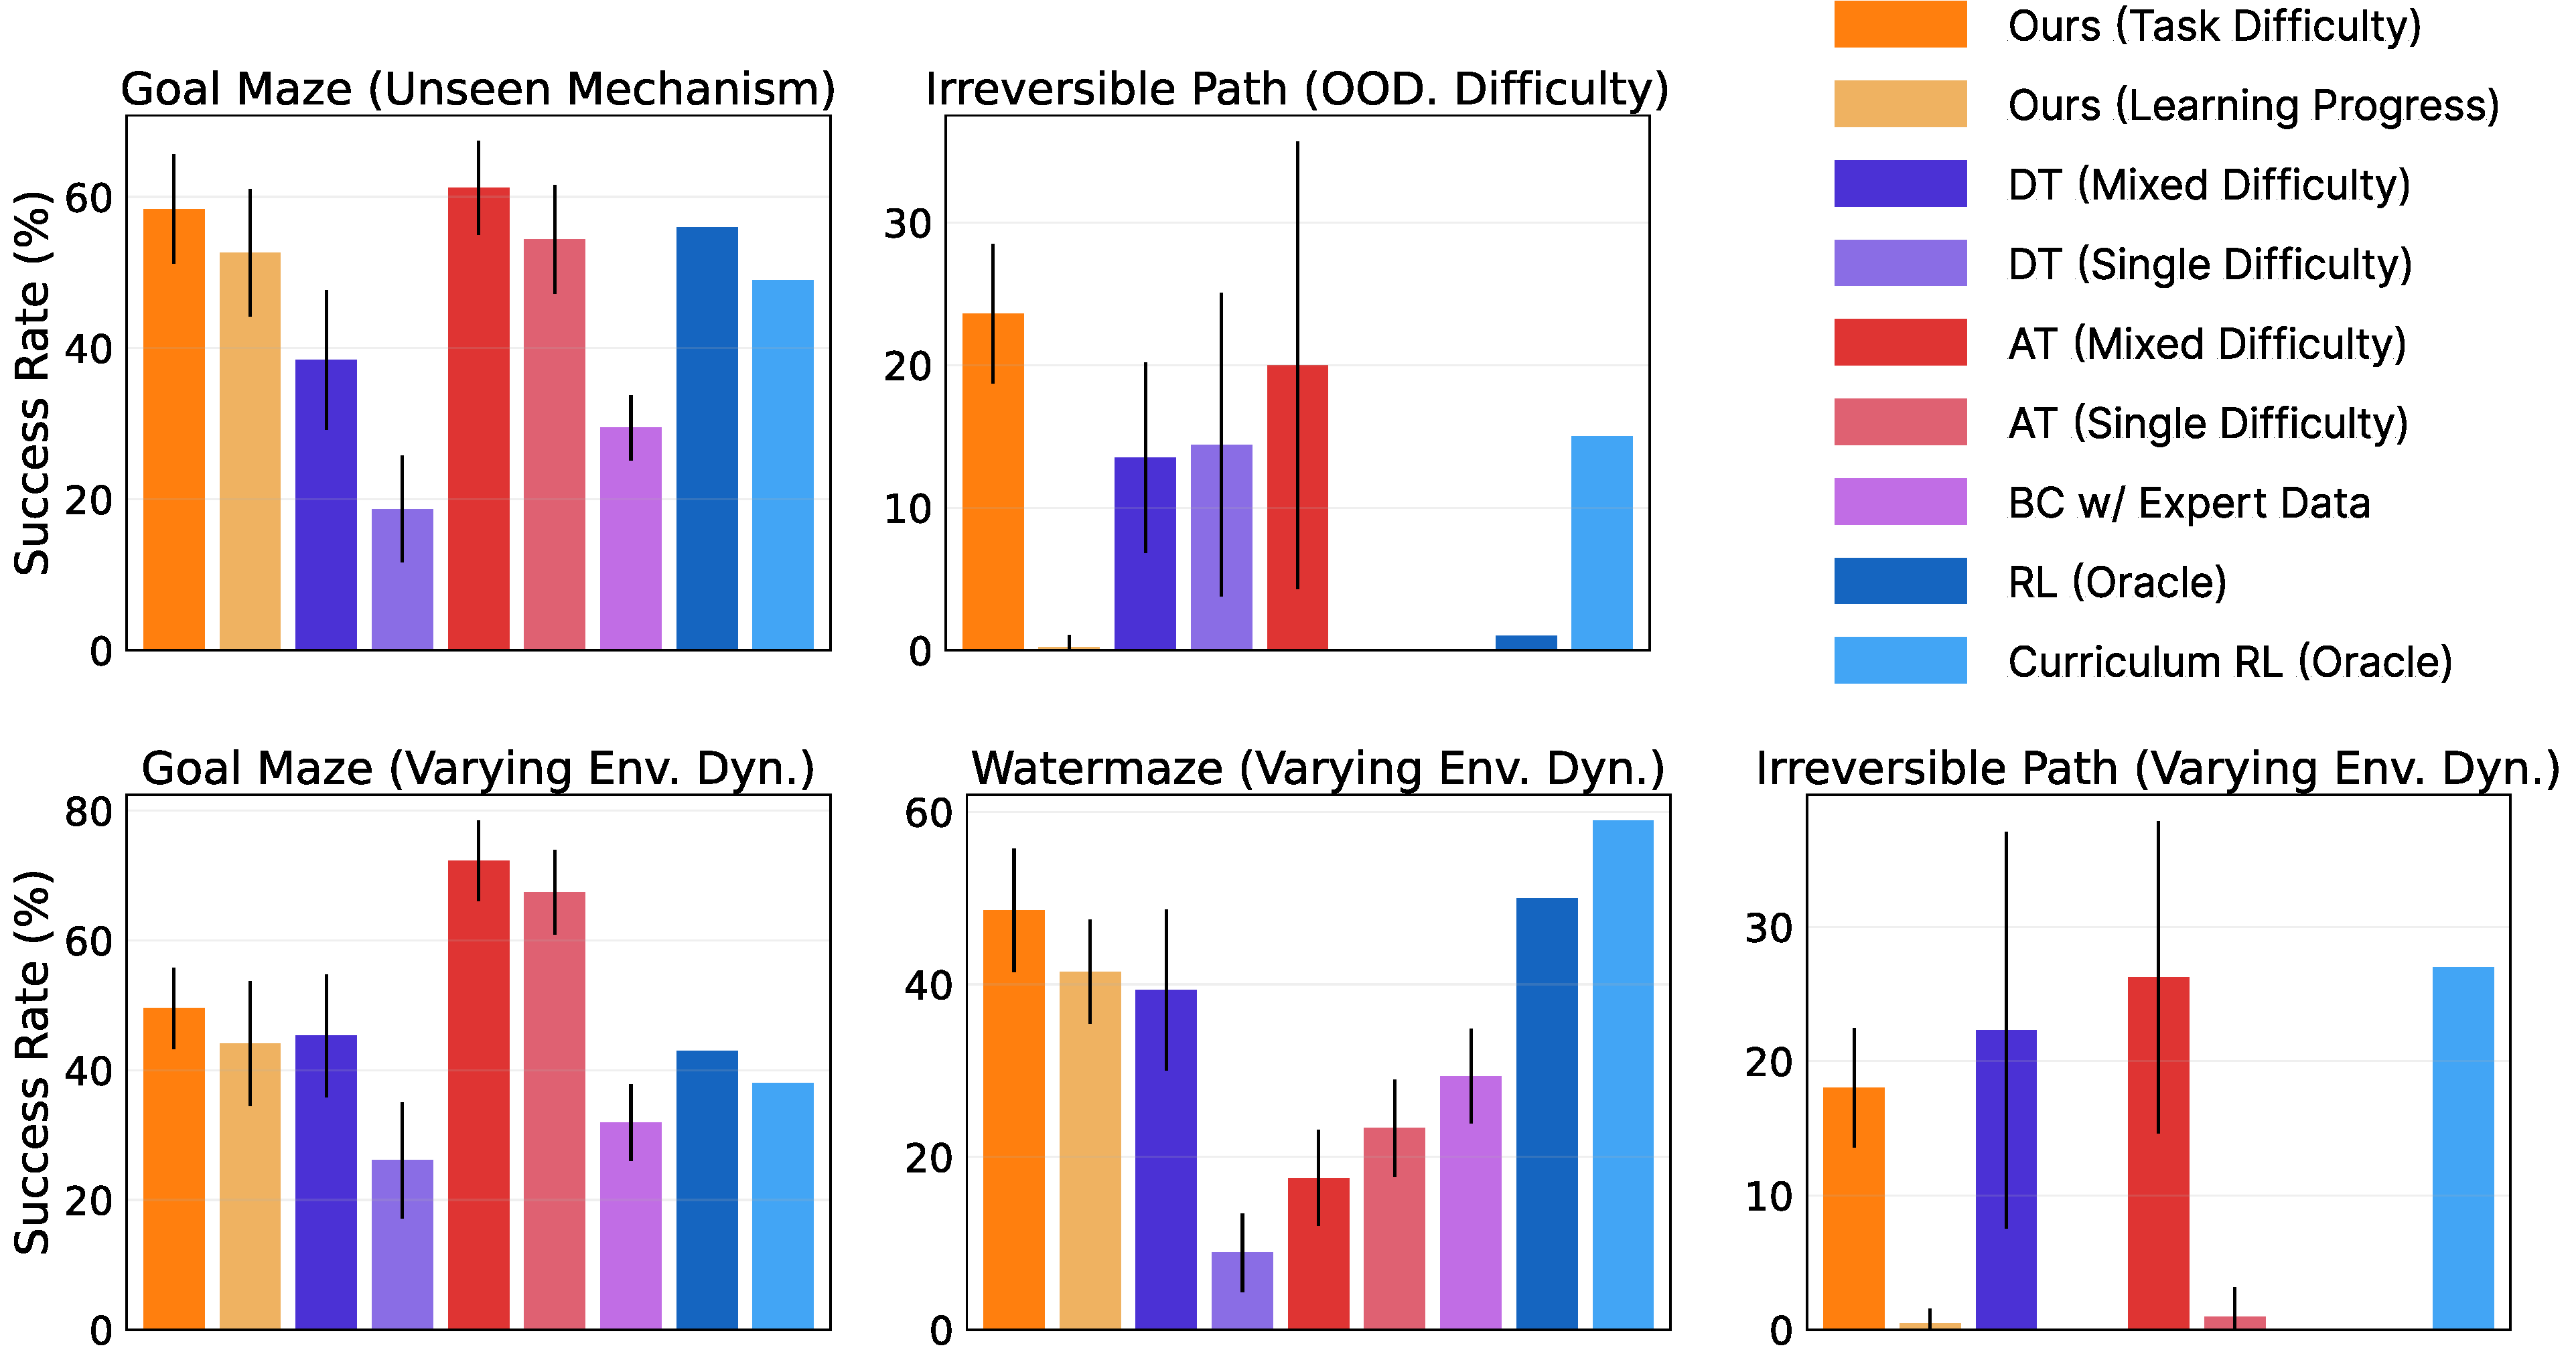
\includegraphics[width=1\textwidth]{fig/dmlab_generalization-fig.pdf}}
    \caption{\textbf{Generalization results on DMLab.} \emph{Top row}: Evaluation results on Goal Maze with unseen maze mechanism and Irreversible Path with out-of-distribution difficulty levels. \emph{Bottom row}: Evaluation results on three levels with environment dynamics differing from training ones. \cec agents display robustness and generalization across various dimensions, outperforming curriculum RL oracles by up to $1.6 \times$. We follow the same evaluation protocol as in Figure~\ref{fig:dmlab_core}. The error bars represent the standard deviations over 20 runs.}
    \label{fig:dmlab_generalization}
    \vspace{-1em}
\end{figure}


\vspace{-0.5em}

\para{Cross-episodic curriculum results in sample-efficient agents.} As shown in Figure~\ref{fig:dmlab_core},  on two out of three examined DMLab levels, \cec agents perform comparable to RL oracles and outperform the BC baselines trained on expert data by at most $2.8\times$.
On the hardest level Irreversible Path where agents have to plan the route ahead and cannot backtrack, both the BC baseline and RL oracle fail.
However, our agents succeed in proposing correct paths that lead to goals and significantly outperform the curriculum RL oracle by $50\%$ even in a \emph{zero-shot} manner.
Because \cec only requires environment interactions generated during the course of training of online source agents (the task-difficulty-based curriculum even contains fewer samples compared to the curriculum RL, as illustrated in Table~\ref{table:dmlab_exp_setting}), the comparable and even better performance demonstrates that our method yields highly sample-efficient embodied policies.
On average, our method with task-difficulty-based curriculum performs the best during evaluation (Table~\ref{supp:table:dmlab_main_avg_results}), confirming the benefit over the concurrent AT approach that leverages chain-of-hindsight experiences. When compared to DT, it outperforms by a significant margin, which suggests that our cross-episodic curriculum helps to squeeze learning signals that are useful for downstream decision-making.

\vspace{-0.5em}

\para{Cross-episodic curriculum boosts the generalization capability.}
To further investigate whether \cec can improve generalization at test time, we construct settings with unseen maze mechanisms (randomly open/closed doors), out-of-distribution difficulty, and different environment dynamics.
See the Appendix, Sec.~\ref{supp:sec:dmlab_generalization} for the exact setups.
As demonstrated in Figure~\ref{fig:dmlab_generalization}, \cec generally improves Transformer agents in learning robust policies that can generalize to perturbations across various axes.
On three settings where the BC w/ Expert Data baseline still manages to make progress, \cec agents are up to $2\times$ better.
Compared to oracle curriculum RL agents, our policies significantly outperform them under three out of five examined scenarios.
It is notable that on Irreversible Path with out-of-distribution difficulty, \cec agent is $1.6\times$ better than the curriculum RL oracle trained on the same data.
These results highlight the benefit of learning with curricular contexts.
On average, our method surpasses the concurrent AT baseline and achieves significantly better performance than other baselines (Table~\ref{supp:table:dmlab_gen_avg_results}). This empirically suggests that CEC helps to learn policies that are robust to environmental perturbations and can quickly generalize to new changes.

\begin{table}[t!]
\caption{\textbf{Evaluation results on RoboMimic.} Visuomotor policies trained with our expertise-based curriculum outperform the most competing history-dependent behavior cloning baseline, as well as other offline RL algorithms. For our method on the Lift task, we conduct 5 independent runs each with 10 rollout episodes. On the Can task, we conduct 10 independent runs each with 5 rollout episodes due to the longer horizon required to complete the task. Standard deviations are included.}
\label{table:robomimic_main}
\vspace{0.1in}
\centering
\resizebox{0.58\textwidth}{!}{
\begin{tabular}{@{}ccccc@{}}
\toprule
\textbf{Task} & \textbf{Ours} & \textbf{BC-RNN}~\citep{mandlekar2021matters}             & \textbf{BCQ}~\citep{fujimoto2018offpolicy}                & \textbf{CQL}~\citep{kumar2020conservative}                \\ \midrule
Lift          &  $\bestscore{100.0 \pm 0.0}$             &    $\bestscore{100.0 \pm 0.0}$                         & $93.3 \pm 0.9$ & $11.3 \pm 9.3$ \\
Can           &   $\bestscore{100.0 \pm 0.0}$            & $\hphantom{\mathbf{0}}96.0 \pm 1.6$ & $77.3 \pm 6.8$ & $\hphantom{0}0.0 \pm 0.0$  \\ \bottomrule
\end{tabular}}

\end{table}


\vspace{-0.5em}

\para{Cross-episodic curriculum is effective across a wide variety of learning scenarios.}
We now move beyond RL settings and study the effectiveness of the expertise-based curriculum in the IL setting with mixed-quality demonstrations.
This is a common scenario, especially in robotics, where demonstrations are collected by human operators with varying proficiency~\citep{mandlekar2018roboturk}.
As presented in Table~\ref{table:robomimic_main}, visuomotor policies trained with the expertise-based curriculum are able to match and outperform the well-established baseline~\citep{mandlekar2021matters} on two simulated robotic manipulation tasks and achieve significantly better performance than agents learned from prevalent offline RL algorithms~\citep{fujimoto2018offpolicy,kumar2020conservative}.
These results suggest that our cross-episodic curriculum is effective and broadly applicable across various problem settings.
More importantly, it provides a promising approach to utilizing limited but sub-optimal data in data-scarce regimes such as robot learning.

\vspace{-0.5em}

\subsection{Ablation Studies}
In this section, we seek to answer the third research question to identify the components critical to the effectiveness of our approach.
We focus on three parts: the importance of cross-episodic attention, the influence of curriculum granularity, and the effect of varying context length.
Finally, we delve into the fourth question, identifying scenarios where CEC is expected to be helpful.

\begin{wrapfigure}{R}{0.4\textwidth}
\vspace{-0.2in}
  \begin{center}
    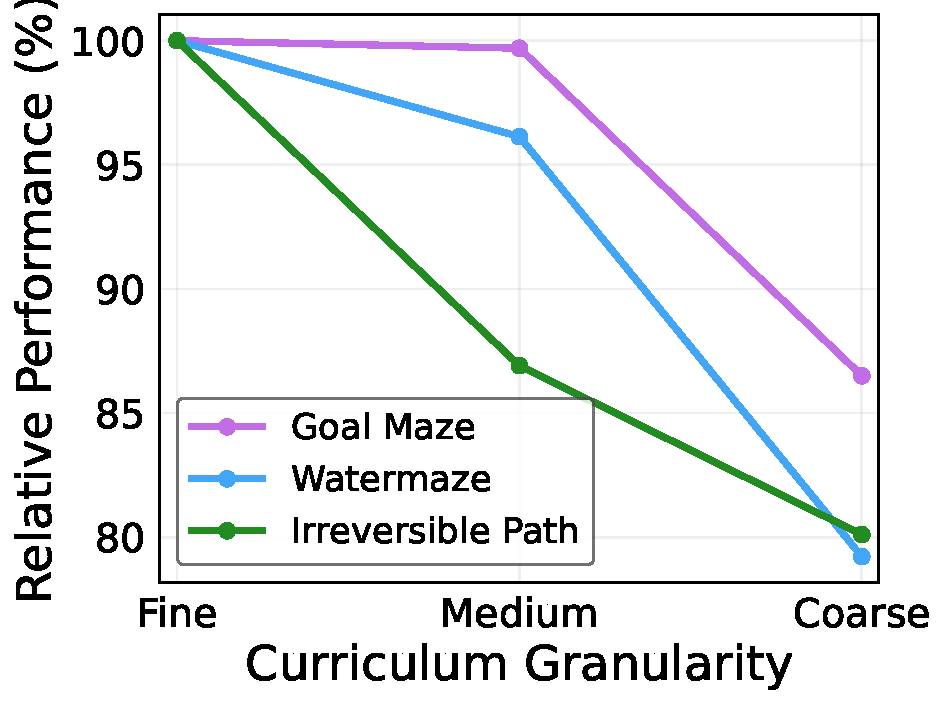
\includegraphics[width=0.4\textwidth]{fig/ablation_curriculum_granularity-fig.pdf}
  \end{center}
      \vspace{-1em}
    \caption{We compare the performance relative to agents trained with the fine-grained curricula. Performance monotonically degrades as task-difficulty-based curricula become coarser.}
    \label{fig:ablation_curriculum_granularity}
\end{wrapfigure}


\begin{table}[t!]
\caption{\textbf{Ablation on the importance of cross-episodic attention.} Transformer agents trained with the same curricular data but without cross-episodic attention degrade significantly during evaluation, suggesting its indispensable role in learning highly performant policies.}
\label{table:ablation_cross_episodic_attention}
\vspace{0.1in}
\centering
\resizebox{1\textwidth}{!}{
\begin{tabular}{@{}r|ccc|cc@{}}
\toprule
\multirow{2}{*}{}                 & \multicolumn{3}{c|}{\textbf{DMLab}}    & \multicolumn{2}{c}{\textbf{RoboMimic}} \\ \cmidrule(l){2-6} 
                                  & Goal Maze   & Watermaze   & Irreversible Path & Lift               & Can               \\ \midrule
Ours                              & $\bestscore{65.2 \pm 6.7}$ & $\bestscore{50.9 \pm 6.6}$ & $\bestscore{38.2 \pm 7.0}$       & $\bestscore{100.0 \pm 0.0}$       & $\bestscore{100.0 \pm 0.0}$      \\
Ours w/o Cross-Episodic Attention & $35.0 \pm 7.1$ & $20.0 \pm 2.5$ & $\hphantom{0}3.8 \pm 4.9$        & $\hphantom{00}75.9 \pm 12.3$       & $\bestscore{\hphantom{0}99.3 \pm 0.9}$       \\ \bottomrule
\end{tabular}

}
\vspace{-1em}
\end{table}


\vspace{-0.5em}

\para{Importance of cross-episodic attention.}
The underlying hypothesis behind our method is that cross-episodic attention enables Transformer agents to distill policy improvement when mixed-optimality trajectories are viewed collectively.
To test this, on DMLab levels and RoboMimic tasks, we train the same Transformer agents with the same curricular data and training epochs but without cross-episodic attention.
We denote such agents as ``\textbf{Ours w/o Cross-Episodic Attention}'' in Table~\ref{table:ablation_cross_episodic_attention}.
Results demonstrate that the ablated variants experience dramatic performance degradation on four out of five examined tasks, which suggests that naively behaviorally cloning sub-optimal data can be problematic and detrimental.
Cross-episodic attention views curricular data collectively, facilitating the extraction of knowledge and patterns crucial for refining decision-making, thereby optimizing the use of sub-optimal data.

\vspace{-0.5em}

\para{Curriculum granularity.} We perform this ablation with the task-difficulty-based curriculum on DMLab levels, due to the ease of adjusting granularity.
We treat the curricula listed in the column ``Ours (Task Difficulty)'' in Table~\ref{table:dmlab_exp_setting} as ``Fine'', and gradually make them coarser to study the impact.
Note that we ensure the same amount of training data.
See the Appendix, Sec.~\ref{supp:sec:curriculum_granularity} for how we define granularity levels ``Medium'' and ``Coarse''.
We visualize the performance relative to the most fine-grained in Figure~\ref{fig:ablation_curriculum_granularity}.
The monotonic degradation of policy performance with respect to curriculum coarseness suggests that fine-grained curricula are critical for Transformer agents to mostly benefit from cross-episodic training.

\begin{wrapfigure}{R}{0.4\textwidth}
\vspace{-2em}
  \begin{center}
    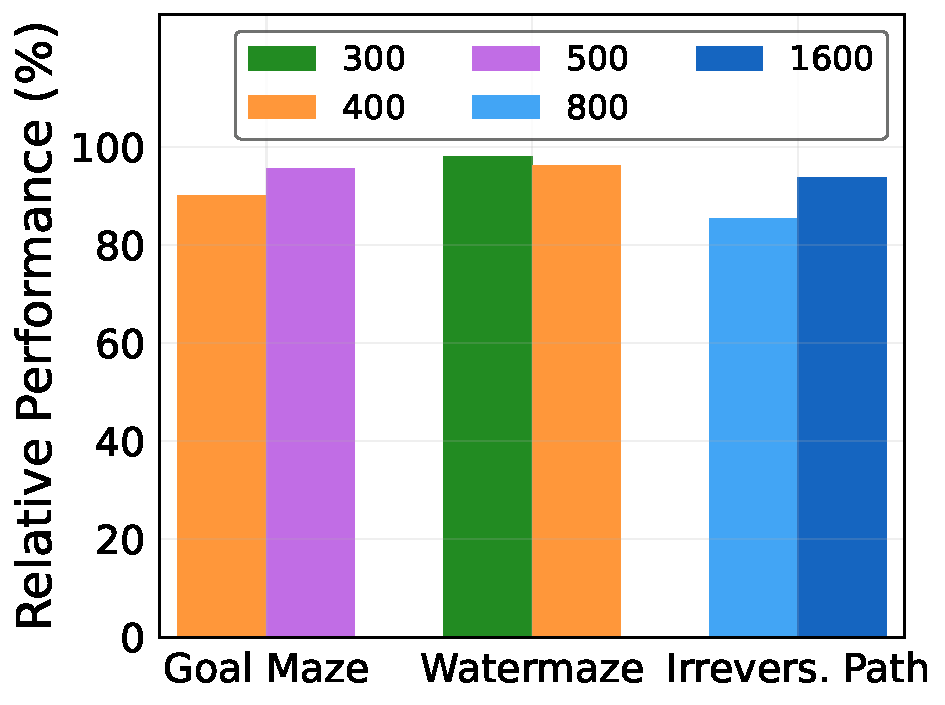
\includegraphics[width=0.4\textwidth]{fig/ablation_horizon-fig.pdf}
  \end{center}
        \vspace{-1em}
    \caption{Both short and unnecessarily long context windows decrease the performance. Numbers in the legend denote context lengths. Performance values are relative to those of ``Ours (Task Difficulty), Auto'' reported in Figure~\ref{fig:dmlab_core}. ``Irrevers. Path'' stands for the task ``Irreversible Path''.}
    \label{fig:ablation_horizon}
    \vspace{-3em}
\end{wrapfigure}


\vspace{-0.5em}

\para{Varying context length.}
Lastly, we study the effect of varying context length on DMLab and visualize it in Figure~\ref{fig:ablation_horizon}.
We normalize all performance values relative to those of ``Ours (Task Difficulty), Auto'' reported in Figure~\ref{fig:dmlab_core}.
It turns out that both too short and unnecessarily long context windows are harmful.
On two out of three levels, using a shorter context decreases the performance even more.
This finding coincides with \citet{laskin2023incontext} that a sufficiently long Transformer context is necessary to retain cross-episodic information.
Furthermore, we also discover that an unnecessarily long context is also harmful.
We hypothesize that this is due to the consequent training and optimization instability.

\para{Curriculum selection based on task complexities and data sources.}
For RL tasks, we recommend starting with the learning-progress-based curriculum. However, if the task itself is too challenging, such that source algorithms barely make progress, we recommend the task-difficulty-based curriculum.
In IL settings, we further investigate the performance of the learning-progress-based curriculum on RoboMimic tasks considered in this work. Detailed setup and results are included in Appendix, Sec~\ref{supp:sec:curriculum_comparison}. To summarize, if human demonstrations are available, even if they are generated to be heterogeneous in quality, we recommend using the expertise-based curriculum. However, in the absence of human demonstrations and only with access to machine-generated data (e.g., generated by RL agents), our learning-progress-based curriculum is recommended because it achieves non-trivial performance and significantly outperforms offline RL methods such as CQL~\citep{kumar2020conservative}. 